\section{MNIST Dataset} \label{sec:prob4}
In this section, we use each of the algorithms to classify handwritten digits from the MNIST dataset.

\subsection{Part 1}
The MNIST dataset contains labeled, handwritten digits.
We split the dataset into multiple classification tasks, shown in the first column of~\cref{table_4_1}.
We also split it into training, validation, and testing sets.

We follow the typical procedure: train with many hyperparameters (C for $L_1$, $L_2$ for LR, and C for SVM), choose the hyperparameters that maximize performance on the validation set with lowest model complexity (low C), and report performance on the test set for the best hyperparameters.

The two classifiers here, Logistic Regression and Linear SVM, perform similarly on each classification task.
For all tasks, the training accuracy was better than the testing accuracy, as expected.

Normalization of the data did not make a large difference ($<\pm 1\%$) for these classifiers, and results presented are for non-normalized data.
The only significant difference after normalization was the size of regularization constant $C$; in all cases, normalization caused the optimal $C$ value to increase by a few orders of magnitude.
This is likely because the size of the data elements decreased, so the size of the learned weight vector increased, meaning a smaller regularization cost had to be applied for the same effect.

A couple misclassified digits are shown in~\cref{fig:misclassified}.
Some handwriting is very difficult even for humans to classify, so it makes sense that our learned classifiers are not perfect.

\begin{figure}\label{fig:misclassified}
    \centering
    \begin{subfigure}[b]{0.5\columnwidth}
        \centering
        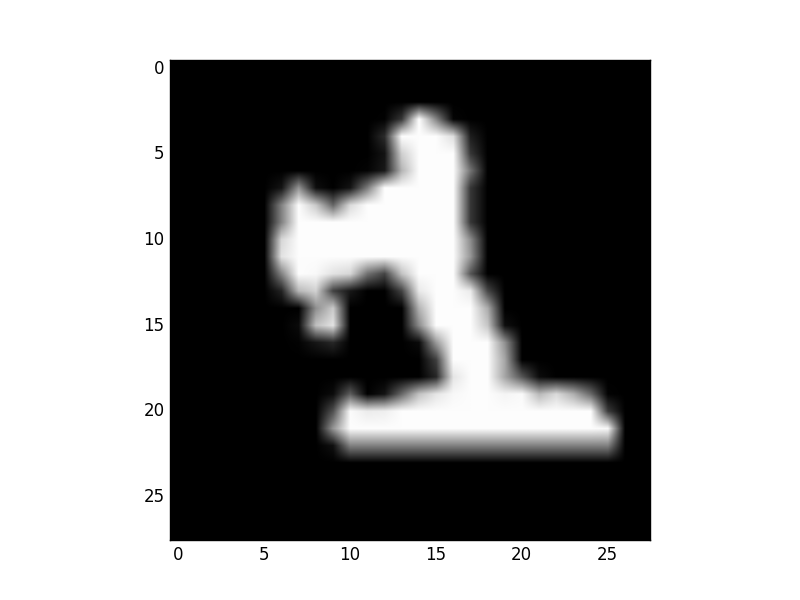
\includegraphics[height=1.2in]{figures/4_1_bad1}
        \caption{Misclassified 1}
    \end{subfigure}%
    ~ 
    \begin{subfigure}[b]{0.5\columnwidth}
        \centering
        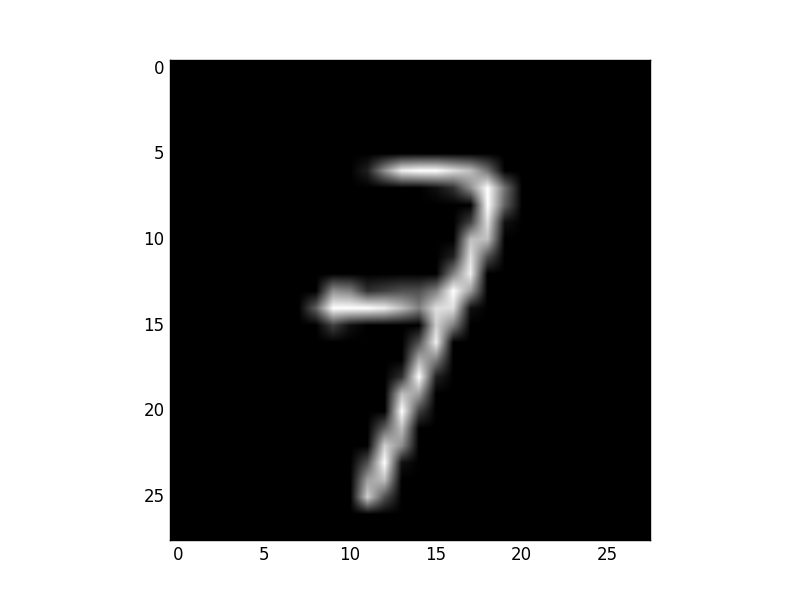
\includegraphics[height=1.2in]{figures/4_1_bad7}
        \caption{Misclassified 7}
    \end{subfigure}
    \caption{The MNIST dataset has some ambiguous entries, in accordance with real human handwriting, that are difficult to classify correctly.}
\end{figure}

\begin{table}[ht!]
\centering
\begin{tabular}{||c c c c c||}  
 \hline
 Dataset & LR Tr. & LR Test & SVM Tr & SVM Test \\ [0.3ex] 
 \hline\hline
 1 vs. 7 & 99.3 & 98.3 ($C=10^{-3}$) & 100.0 & 98.3 ($C=10^{-6}$) \\ 
 \hline
 3 vs. 5 & 100.0 & 93.3 ($C=10^{-1}$) & 100.0 & 93.6 ($C=10^{-1}$) \\ 
 \hline
 4 vs. 9 & 100.0 & 94.7 ($C=10^{0}$) & 100.0 & 94.0 ($C=10^{0}$) \\ 
 \hline
 odds vs. evens & 100.0 & 84.5 ($C=10^{2}$) & 98.3 & 84.3 ($C=10^{-1}$) \\ 
 \hline
\end{tabular}
\caption{Accuracy of LR and Linear SVM on MNIST datasets.}
\label{table_4_1}
\end{table}

\subsection{Part 2}
[todo]

\begin{table}[ht!]
\centering
\begin{tabular}{||c c c c c||}  
 \hline
 Dataset & LR Tr. & LR Test & SVM Tr & SVM Test \\ [0.3ex] 
 \hline\hline
 1 vs. 7 & 99.3 & 98.3 ($C=10^{-3}, \lambda=$) \\ 
 \hline
 3 vs. 5 & 100.0 & 93.3 ($C=10^{-1}$) & 100.0 & 93.6 ($C=10^{-1}$) \\ 
 \hline
 4 vs. 9 & 100.0 & 94.7 ($C=10^{0}$) & 100.0 & 94.0 ($C=10^{0}$) \\ 
 \hline
 odds vs. evens & 100.0 & 84.5 ($C=10^{2}$) & 98.3 & 84.3 ($C=10^{-1}$) \\ 
 \hline
\end{tabular}
\caption{Accuracy of Gaussian RBF SVM classifier on MNIST datasets.}
\label{table_4_2}
\end{table}

\subsection{Part 3}
[todo]

